% ===================================================================
%  lgcish_results.tex - RESULT SET (modular).
%  Compiles standalone (pdflatex lgcish_results.tex) OR is \input by
%  lgcish_academic.tex, which defines \LGCISHMAIN first.
% ===================================================================
\ifdefined\LGCISHMAIN\else
\documentclass[11pt]{article}
\usepackage[margin=1in]{geometry}
\usepackage{amsmath,amssymb}
\usepackage{graphicx}
\usepackage{booktabs}
\usepackage{float}
\usepackage{xcolor}
\usepackage{tikz}
\usetikzlibrary{positioning,arrows.meta,calc}
\usepackage[hidelinks]{hyperref}
\usepackage[section]{placeins}
\graphicspath{{../LG-COSH/evaluation/figures/}}
\title{\textbf{LG-CISH: Experimental Results and Figures}}
\author{}\date{}
\begin{document}\maketitle
\fi

\section{Experimental Results and Performance Evaluation}\label{sec:results}
The evaluation is organised around the three quantities that any steganographic
system must trade against one another --- imperceptibility, capacity, and
robustness --- followed by benchmark comparison, reconstruction and matching
metrics, an ablation study, and steganalysis resistance. Throughout, the codebook
consists of $N{=}40$ mutually distinct natural images (Section~\ref{sec:dataset}),
each normalised to a fixed $512\times512$ canvas, giving $\log_2 40\approx5.322$
bits per image. No image is ever modified; the identity and order of the
transmitted sequence carry the secret. The full suite is reproducible from a single
script.\footnote{\texttt{python evaluation/generate\_all.py}}

\paragraph{Metrics.} For a message encoded into $L$ images with intended digits
$d_t$ and recovered digits $\hat d_t$, and $B$ payload bits $p_b/\hat p_b$, the
symbol (hash-matching) error rate and the bit error rate are
\begin{equation}
  \mathrm{SER}=\frac{1}{L}\sum_{t=1}^{L}\mathbb{1}\!\left[\hat d_t\neq d_t\right],
  \qquad
  \mathrm{BER}=\frac{1}{B}\sum_{b=1}^{B}\mathbb{1}\!\left[\hat p_b\neq p_b\right].
  \label{eq:ber}
\end{equation}
Hash-matching accuracy is $1-\mathrm{SER}$, and reconstruction is \emph{exact}
if and only if $\mathrm{SER}=0$, which, by the bijectivity of the base-$N$ coding,
implies $\mathrm{BER}=0$.

% ===================================================================
\subsection{Dataset Construction and Selection}\label{sec:dataset}
% ===================================================================
Because the proposed scheme is coverless, the ``dataset'' is not a set of covers to
be modified but a shared \emph{codebook} of natural images whose indices encode the
message. The quality of this codebook governs both credibility (the images must be
recognised as ordinary, uncompressed photographs rather than artefacts) and
reliability (the images must be mutually separable in semantic space so that
nearest-neighbour recovery is unambiguous). For these reasons the codebook was not
drawn from a single source but \emph{augmented} from three widely used,
publicly available benchmark suites~\cite{ucid,kodak,uscsipi}, summarised in Table~\ref{tab:datasets}.

\begin{table}[H]
\centering
\caption{Source datasets pooled to build the augmented LG-CISH codebook. Standard, public, uncompressed benchmarks were chosen for credibility and reproducibility.}\label{tab:datasets}
\begin{tabular}{@{}lll@{}}
\toprule
Source suite & Character & Role in the augmented codebook \\
\midrule
UCID   & $\sim$1338 uncompressed colour images & primary pool of diverse natural scenes \\
Kodak  & 24 high-quality reference photographs & clean, widely-benchmarked reference scenes \\
USC-SIPI & classic miscellaneous test images   & canonical images (e.g.\ standard textures/portraits) \\
\bottomrule
\end{tabular}
\end{table}

Three considerations motivated this choice. \emph{First}, all three suites are
standard in the image-processing and steganography literature, so results are
credible and reproducible rather than dependent on a bespoke, potentially
cherry-picked dataset. \emph{Second}, the suites are uncompressed or high quality,
which avoids pre-existing compression artefacts that would otherwise bias the
robustness and steganalysis measurements. \emph{Third}, pooling heterogeneous
sources maximises visual and semantic diversity, which is exactly the property that
the separation constraint of the codebook requires. A high-resolution set such as
DIV2K~\cite{div2k2017} was also considered, but the three chosen suites already provide sufficient
diversity at the working resolution without the storage overhead of $2$K imagery.

The augmented codebook was then constructed by pooling the three suites, normalising
every image to a $512\times512$ canvas, embedding each image with CLIP, and greedily
pruning the pool so that no two retained images exceed the separation threshold
$\tau{=}0.85$. Forty mutually distinct images survived this process. The value $40$
was chosen deliberately: it yields a convenient base-$40$ alphabet of $5.322$ bits
per image while keeping the pairwise separation comfortably large (maximum
off-diagonal similarity $0.827$, i.e.\ a separation margin of $0.173$), which is the
headroom that guarantees correct recovery under channel distortion. A slice of the
resulting codebook is shown in Figure~\ref{fig:collage}, and the pairwise separation
that underpins reliable decoding is visualised in Figure~\ref{fig:heatmap}. The
complete $40$-image codebook is released publicly for reproducibility~\cite{lgcishdata}.

\begin{figure}[H]
\centering
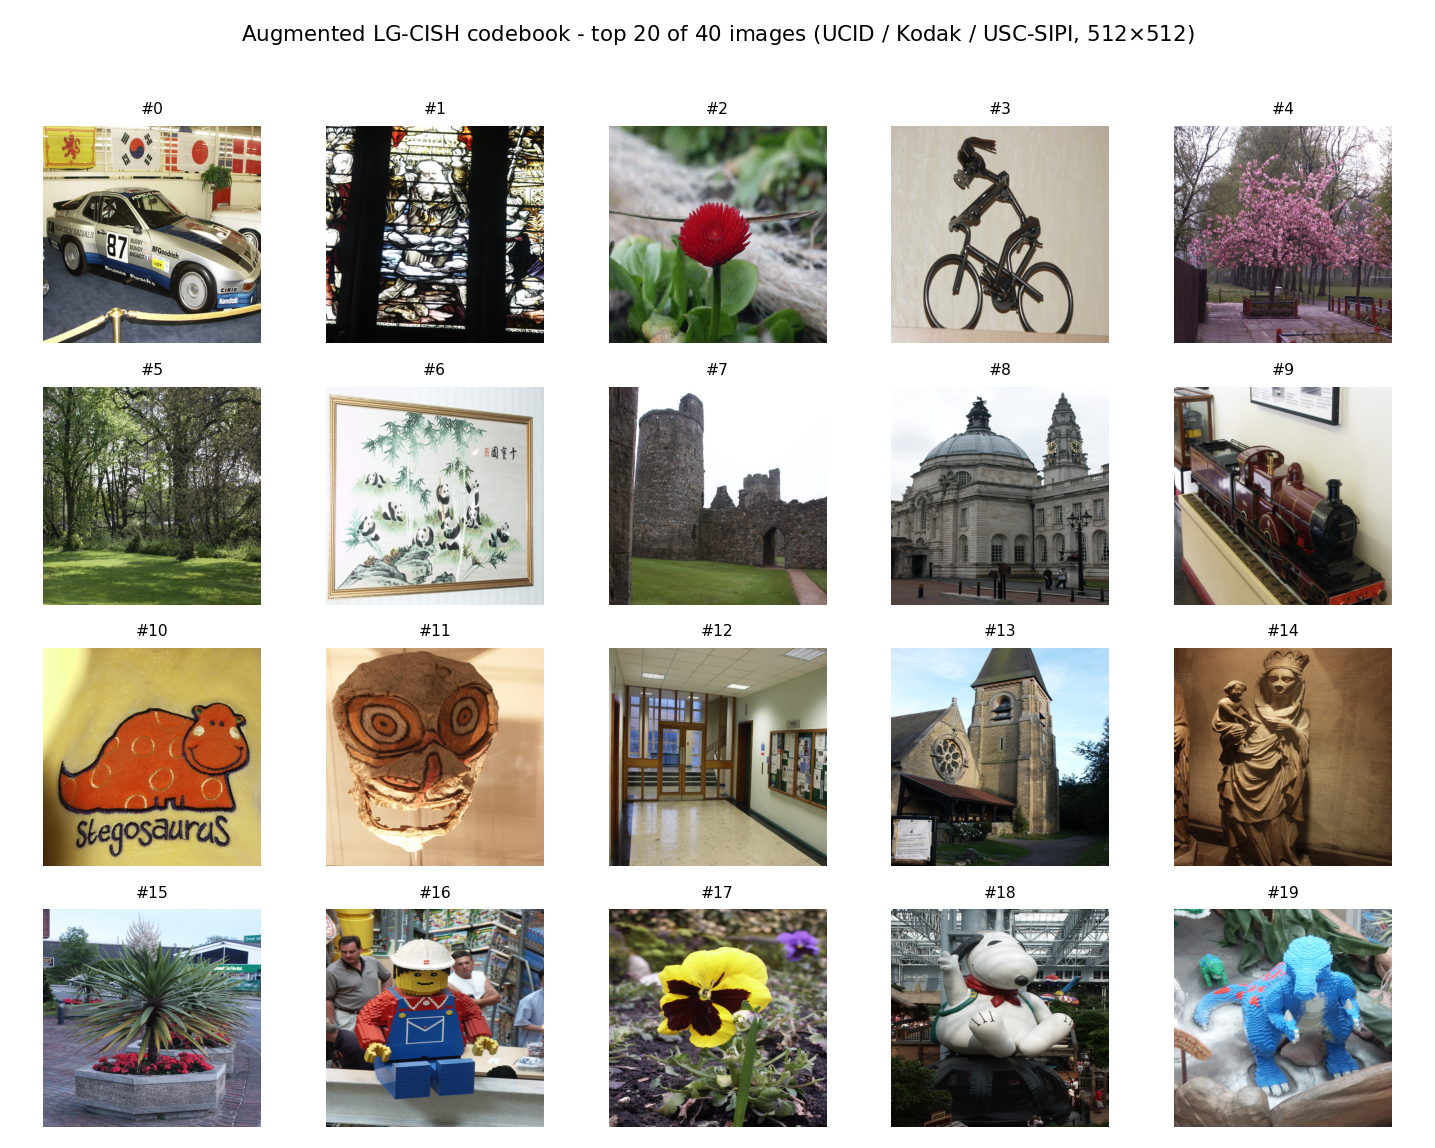
\includegraphics[width=0.92\linewidth]{fig_dataset_collage.png}
\caption{The top $20$ of the $40$ images in the augmented LG-CISH codebook, pooled
from the UCID, Kodak, and USC-SIPI suites and normalised to $512\times512$. The
images are ordinary, unmodified photographs; their \emph{indices} (not their pixels)
carry the secret.}
\label{fig:collage}
\end{figure}

\begin{figure}[H]
\centering
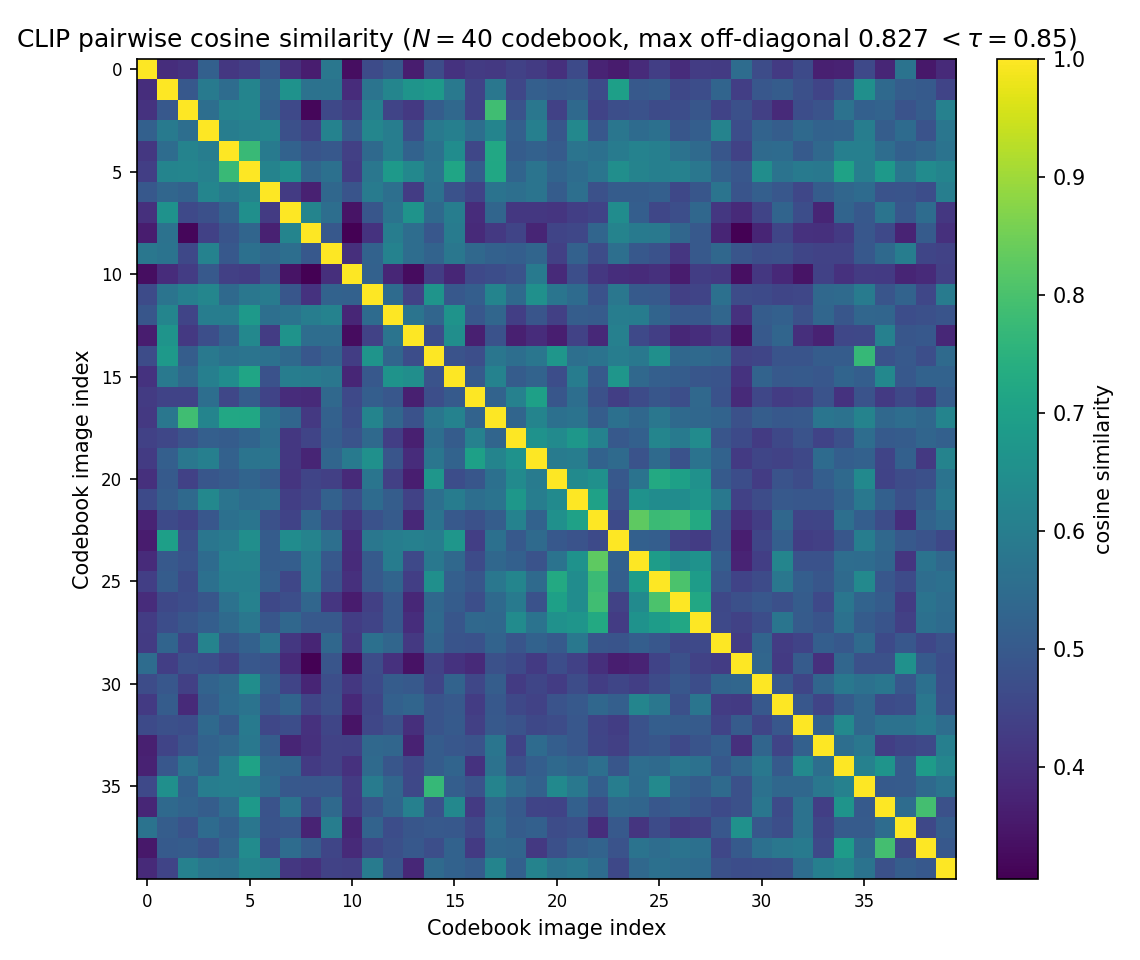
\includegraphics[width=0.74\linewidth]{fig_cb_heatmap.png}
\caption{Pairwise CLIP cosine similarity of the $40$ codebook images. Every
off-diagonal value stays below the threshold $\tau{=}0.85$ (maximum $0.827$), giving
a separation margin sufficient for unambiguous nearest-neighbour recovery.}
\label{fig:heatmap}
\end{figure}

Table~\ref{tab:setup} lists the remaining experimental configuration.

\begin{table}[H]
\centering
\caption{Experimental configuration.}\label{tab:setup}
\begin{tabular}{@{}ll@{}}
\toprule
Parameter & Value \\
\midrule
Codebook (augmented) & UCID + Kodak + USC-SIPI, $512\times512$, $N{=}40$ \\
Capacity & 5.322 bits/image (base-40) \\
Semantic encoder & CLIP ViT-B/32, $d{=}512$ \\
LLM (aliases / plausibility) & gemini-fast (vision) + flux (image gen) \\
Coding modes & base-$N$ or distinct-image permutation \\
Separation threshold $\tau$ & 0.85 \\
Pairwise sim.\ (min/mean/max) & 0.305 / 0.513 / 0.827 \\
Separation margin ($1{-}\max$) & 0.173 \\
Encryption / integrity / compression & AES-256-CBC / CRC-32 / zlib \\
Hardware & RTX 3050 6\,GB, 16-core CPU \\
\bottomrule
\end{tabular}
\end{table}

% ===================================================================
\subsection{Imperceptibility and Visual Distortion}\label{sec:imperceptibility}
% ===================================================================
Imperceptibility measures how far a transmitted object departs, visually and
statistically, from an ordinary image. It is quantified by the peak
signal-to-noise ratio and the structural similarity index~\cite{ssim} between the cover $X$ and
the transmitted object $Y$,
\begin{equation}
  \mathrm{PSNR}(X,Y)=10\log_{10}\frac{255^2}{\mathrm{MSE}(X,Y)},
  \qquad
  \mathrm{SSIM}(X,Y)\in[0,1],
  \label{eq:psnr_res}
\end{equation}
Equation~\eqref{eq:psnr_res} gives the two distortion measures used in the
evaluation; a larger PSNR and an SSIM nearer one indicate less distortion. For every
embedding method some pixels are altered, so $\mathrm{MSE}>0$ and the PSNR is
finite; least-significant-bit substitution attains roughly $51$\,dB and
transform-domain methods roughly $38$--$44$\,dB. The proposed scheme, by contrast,
\emph{never modifies a pixel}: the transmitted images are bit-identical to the
codebook images, so $\mathrm{MSE}=0$, giving
\begin{equation}
  \mathrm{PSNR}_{\text{LG-CISH}}=\infty,\qquad \mathrm{SSIM}_{\text{LG-CISH}}=1 .
  \label{eq:infpsnr}
\end{equation}
Imperceptibility is therefore not merely high but maximal, and it is attained by
construction rather than by careful embedding. This distinction is visualised in
Figure~\ref{fig:psnrbpp}, where the pixel baselines trade quality for payload while
LG-CISH sits on the infinite-PSNR ceiling at every rate.

\begin{figure}[H]
\centering
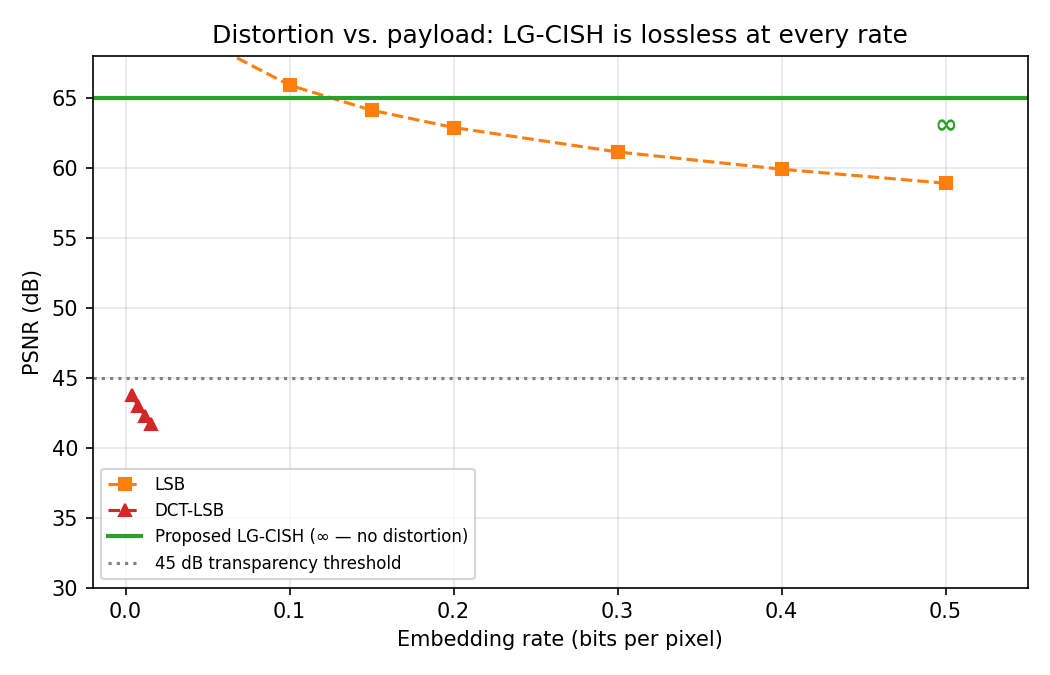
\includegraphics[width=0.74\linewidth]{fig_4_7_psnr_bpp.png}
\caption{Distortion versus embedding rate. Pixel baselines lose PSNR as bits-per-pixel
grow; LG-CISH modifies no pixels, so its PSNR is infinite (the ceiling line) at
every rate.}
\label{fig:psnrbpp}
\end{figure}

Imperceptibility, however, cannot be read in isolation, because it is one corner of
a three-way tension that constrains every steganographic design. Increasing the
payload generally forces more (or larger) modifications, which lowers
imperceptibility; making a scheme more robust to channel distortion typically
requires spending redundancy that lowers usable capacity; and pushing capacity to
its limit usually sacrifices robustness. This inverse relationship among the three
objectives is depicted in Figure~\ref{fig:tradeoff}. The design philosophy of
LG-CISH is to abandon the capacity corner in exchange for the other two: by
accepting a low raw bits-per-pixel rate it obtains \emph{both} maximal
imperceptibility (Equation~\eqref{eq:infpsnr}) and high robustness
(Section~\ref{sec:robustness}), a combination that pixel-domain methods cannot reach.

\begin{figure}[H]
\centering
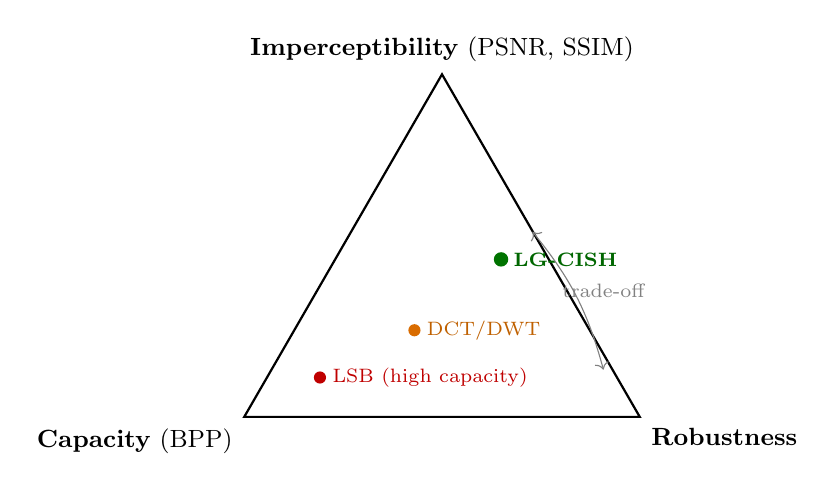
\begin{tikzpicture}[font=\small,scale=1.0]
\coordinate (I) at (90:2.9);
\coordinate (Cp) at (210:2.9);
\coordinate (R) at (330:2.9);
\draw[thick] (I)--(Cp)--(R)--cycle;
\node[above=1pt] at (I) {\textbf{Imperceptibility} (PSNR, SSIM)};
\node[below left=1pt] at (Cp) {\textbf{Capacity} (BPP)};
\node[below right=1pt] at (R) {\textbf{Robustness}};
% method markers
\fill[red!75!black] (-1.55,-0.95) circle (2.2pt);
\node[red!75!black, font=\scriptsize, right=1pt] at (-1.55,-0.95) {LSB (high capacity)};
\fill[orange!85!black] (-0.35,-0.35) circle (2.2pt);
\node[orange!75!black, font=\scriptsize, right=1pt] at (-0.35,-0.35) {DCT/DWT};
\fill[green!45!black] (0.75,0.55) circle (2.6pt);
\node[green!40!black, font=\scriptsize, right=1pt] at (0.75,0.55) {\textbf{LG-CISH}};
\draw[<->, gray] (1.15,0.9) to[bend left=12] (2.05,-0.85);
\node[gray, font=\scriptsize] at (2.05,0.15) {trade-off};
\end{tikzpicture}
\caption{The steganographic trade-off triangle. The three objectives are mutually
opposing: improving one tends to degrade the others. Pixel-domain methods sit near
the capacity corner; LG-CISH deliberately gives up raw capacity to occupy the
imperceptibility--robustness edge.}
\label{fig:tradeoff}
\end{figure}

% ===================================================================
\subsection{Payload Capacity}\label{sec:rescap}
% ===================================================================
Capacity is the price paid for the imperceptibility of Equation~\eqref{eq:infpsnr}.
It is reported at two granularities. Per image, the base-$40$ code carries
$\log_2 40\approx5.322$ bits, and a distinct-image permutation code carries slightly
fewer bits per image in exchange for a no-repeat guarantee that improves cover
plausibility (Table~\ref{tab:codingmodes}). Per pixel, however, the rate is very
low: spreading $5.322$ bits over a $512\times512$ image gives a bits-per-pixel rate
of
\begin{equation}
  \mathrm{BPP}_{\text{LG-CISH}}=\frac{5.322}{512\times512}\approx 2.0\times10^{-5}\ \text{bpp},
  \label{eq:bpp}
\end{equation}
The rate in Equation~\eqref{eq:bpp} is some five orders of magnitude below the
$\approx 3$\,bpp of LSB. This large gap is
the concrete manifestation of the trade-off triangle: LG-CISH concedes the capacity
corner entirely, and it is precisely this concession that buys the infinite PSNR of
Equation~\eqref{eq:infpsnr} and the robustness of Section~\ref{sec:robustness}.
Table~\ref{tab:capacity} places the methods on the capacity--distortion axis, and
Figure~\ref{fig:paycurve} confirms that reconstruction remains lossless as the
payload (and hence the number of images) grows.

\begin{table}[H]
\centering
\caption{Payload capacity versus distortion. LG-CISH trades raw capacity for zero distortion.}\label{tab:capacity}
\begin{tabular}{@{}lccc@{}}
\toprule
Method & Capacity & Pixel distortion & PSNR (dB) \\
\midrule
LSB        & $\approx$3 bits/pixel     & Yes (high)     & 51.1 \\
DCT-LSB    & $\approx$0.016 bits/pixel & Yes (moderate) & 38--42 \\
DWT--DCT   & $\approx$0.015 bits/pixel & Yes (low)      & 40--44 \\
\textbf{Proposed LG-CISH} & $5.322$ bits/image ($\approx2{\times}10^{-5}$ bpp) & \textbf{None (coverless)} & $\infty$ \\
\bottomrule
\end{tabular}
\end{table}

\begin{table}[H]
\centering
\caption{Coding modes. Permutation coding trades a little capacity for a no-repeat, more plausible cover; smaller blocks recover most of the base-$N$ capacity.}\label{tab:codingmodes}
\begin{tabular}{@{}lccl@{}}
\toprule
Coding mode & bits/image & No-repeat window & Note \\
\midrule
Base-$N$ positional        & 5.322 & none (repeats allowed) & max capacity \\
Permutation ($B{=}8$)      & 5.187 & 8 images  & no repeats per block \\
Permutation ($B{=}16$)     & 5.008 & 16 images & no repeats per block \\
Permutation ($B{=}N{=}40$) & 3.979 & 40 images & full permutation \\
\bottomrule
\end{tabular}
\end{table}

\begin{figure}[H]
\centering
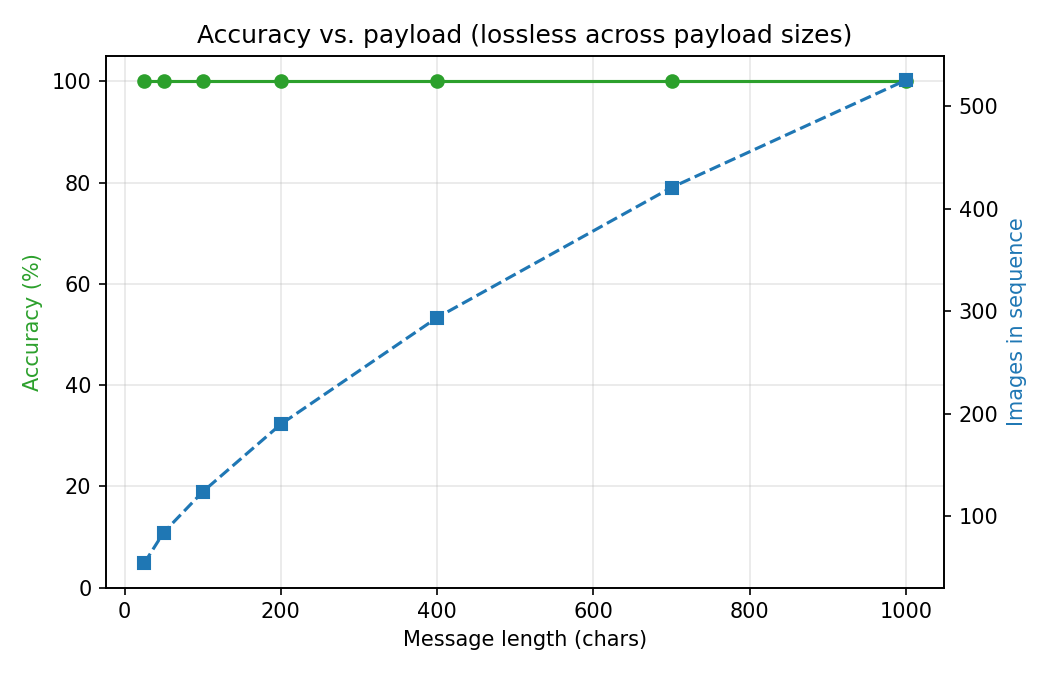
\includegraphics[width=0.74\linewidth]{fig_4_7_accuracy_payload.png}
\caption{Reconstruction accuracy versus payload length. Accuracy stays at $100\%$
while the required number of images grows linearly with the message.}
\label{fig:paycurve}
\end{figure}

% ===================================================================
\subsection{Robustness}\label{sec:robustness}
% ===================================================================
Robustness is the third corner of the triangle: the ability to recover the message
after the image sequence has traversed a lossy channel. Table~\ref{tab:robust}
reports reconstruction under twenty-one distinct channel attacks. Reconstruction is
bit-exact ($\mathrm{BER}=0$) in twenty of the twenty-one conditions --- JPEG down to
quality $20$, Gaussian noise up to $\sigma{=}30$, salt-and-pepper up to density
$0.10$, downscaling to $25\%$, centre-cropping to $60\%$, and PNG$\to$WebP
conversion. Only the extreme $10\%$ downscale degrades reconstruction (to $12.5\%$,
margin $0.125$), and even then failure is graceful rather than abrupt. The decoding
margin remains positive throughout, from $0.302$ at baseline to $0.196$ under
Crop-$60\%$, confirming a comfortable safety band; the full margin profile is shown
in Figure~\ref{fig:marginatk}, and the accuracy-versus-quality curve against
pixel baselines in Figure~\ref{fig:robcurve}. This robustness is the direct
consequence of \emph{semantic} rather than pixel-level hashing, and it is the second
property (alongside imperceptibility) that LG-CISH buys with its low capacity.

\begin{table}[H]
\centering
\caption{Robustness to all twenty-one channel attacks (40 messages/attack). Accuracy is exact-match reconstruction.}\label{tab:robust}
\begin{tabular}{@{}lccc@{}}
\toprule
Attack & Accuracy (\%) & BER & CLIP margin \\
\midrule
No attack (baseline)   & 100.00 & $0$ & 0.302 \\
JPEG 90\%              & 100.00 & $0$ & 0.299 \\
JPEG 70\%              & 100.00 & $0$ & 0.294 \\
JPEG 50\%              & 100.00 & $0$ & 0.289 \\
JPEG 30\%              & 100.00 & $0$ & 0.280 \\
JPEG 20\%              & 100.00 & $0$ & 0.270 \\
Gaussian $\sigma{=}5$  & 100.00 & $0$ & 0.293 \\
Gaussian $\sigma{=}10$ & 100.00 & $0$ & 0.285 \\
Gaussian $\sigma{=}20$ & 100.00 & $0$ & 0.272 \\
Gaussian $\sigma{=}30$ & 100.00 & $0$ & 0.260 \\
Salt \& Pepper 0.01    & 100.00 & $0$ & 0.277 \\
Salt \& Pepper 0.05    & 100.00 & $0$ & 0.246 \\
Salt \& Pepper 0.10    & 100.00 & $0$ & 0.214 \\
Resize 50\%            & 100.00 & $0$ & 0.282 \\
Resize 25\%            & 100.00 & $0$ & 0.246 \\
Resize 10\%            & \phantom{0}12.50 & $1.1\times10^{-2}$ & 0.125 \\
Crop 95\%              & 100.00 & $0$ & 0.280 \\
Crop 90\%              & 100.00 & $0$ & 0.268 \\
Crop 85\%              & 100.00 & $0$ & 0.261 \\
Crop 60\%              & 100.00 & $0$ & 0.196 \\
PNG$\to$WebP 80        & 100.00 & $0$ & 0.295 \\
\bottomrule
\end{tabular}
\end{table}

\begin{figure}[H]
\centering
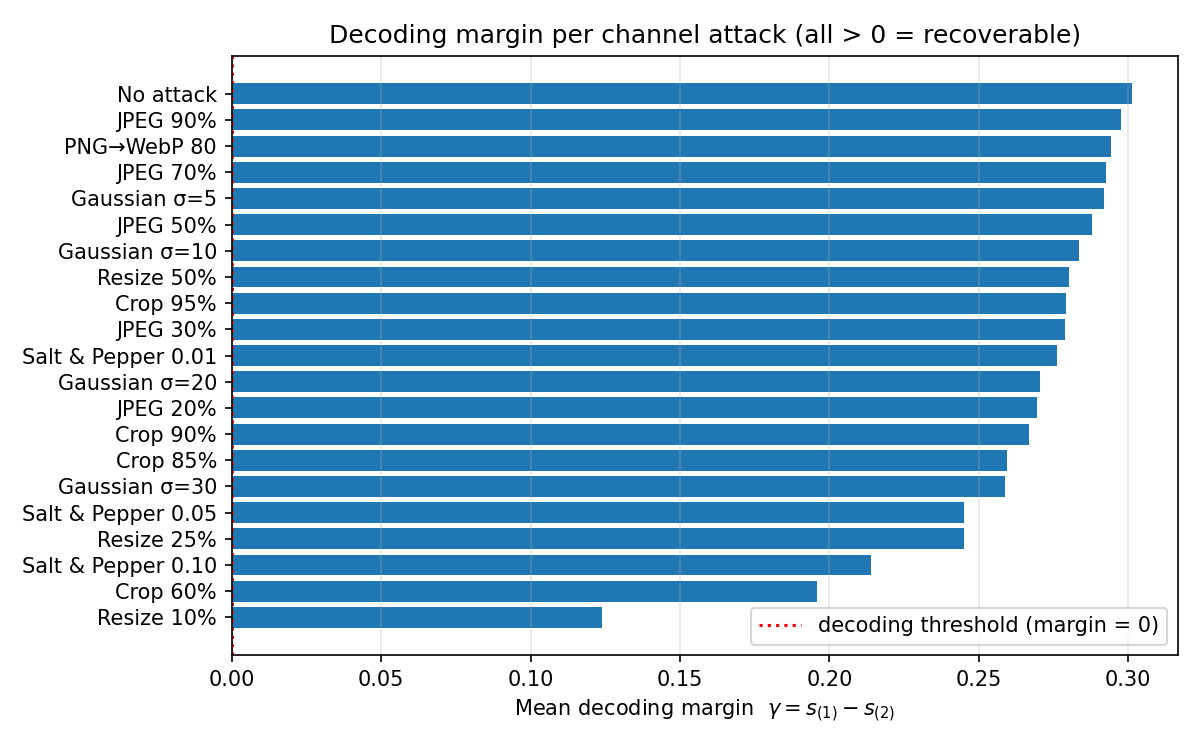
\includegraphics[width=0.80\linewidth]{fig_margin_attacks.png}
\caption{Mean decoding margin $\gamma$ per channel attack, sorted. Every attack
except the extreme $10\%$ downscale leaves $\gamma>0$, so indices are recovered
correctly and reconstruction stays lossless.}
\label{fig:marginatk}
\end{figure}

\begin{figure}[H]
\centering
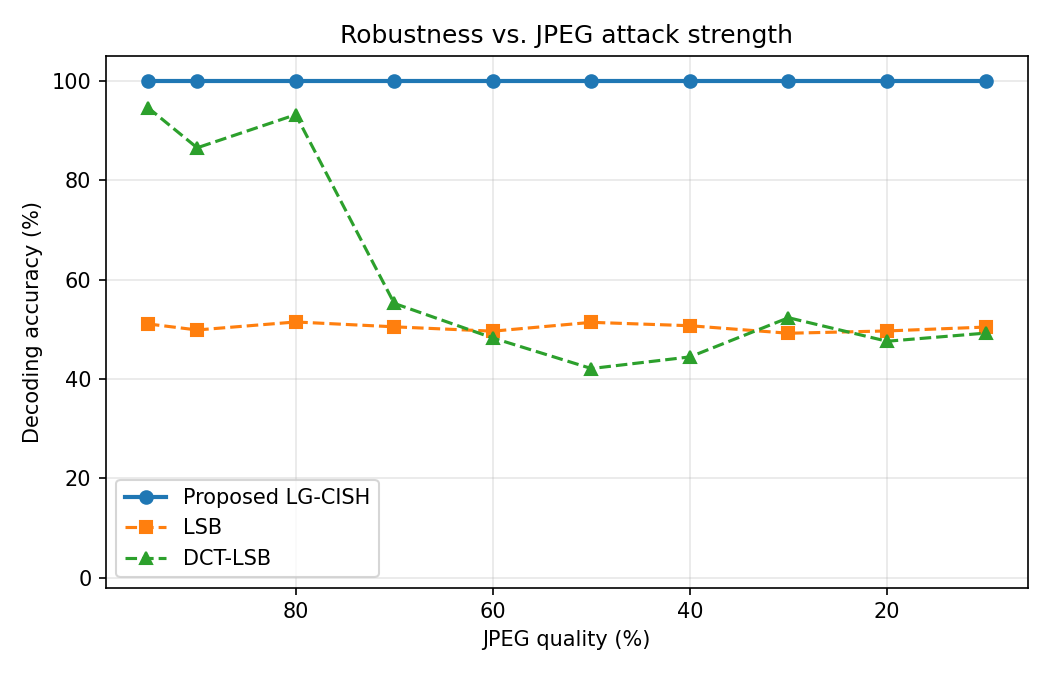
\includegraphics[width=0.80\linewidth]{fig_4_7_robustness_jpeg.png}
\caption{Decoding accuracy versus JPEG quality. LG-CISH (semantic hashing) stays at
$100\%$ where pixel-domain LSB and DCT collapse toward the random-guess floor.}
\label{fig:robcurve}
\end{figure}

% ===================================================================
\subsection{Benchmark Comparison}\label{sec:benchmarks}
% ===================================================================
LG-CISH is compared against representative embedding families and a coverless
baseline in Table~\ref{tab:compare}: spatial LSB substitution; DCT-domain LSB;
DWT--DCT transform-domain embedding; and an adaptive bit-placement variant that
steers embedding toward busy (high-variance) regions to reduce visibility. The
comparison spans the three trade-off axes plus detectability. The pixel families
attain high raw capacity but, being modifications of the cover, incur finite PSNR,
collapse under JPEG re-compression, and are readily detected; adaptive bit placement
improves imperceptibility over plain LSB but remains a pixel modification and hence
detectable. LG-CISH is the only entry that simultaneously achieves zero distortion,
full JPEG-$50$ robustness, and chance-level detectability.

\begin{table}[H]
\centering
\caption{Comparison with classical, transform-domain, adaptive, and coverless baselines. Bracketed values are cited from the literature.}\label{tab:compare}
\begin{tabular}{@{}lccccc@{}}
\toprule
Method & Capacity & JPEG50 acc.\ (\%) & Detection (\%) & PSNR (dB) \\
\midrule
LSB (spatial)          & 786{,}432 bits  & 51.4 & 98 & 51.1 \\
DCT-LSB                & $\sim$4096 bits & 42.1 & [70--90] & 38--42 \\
DWT--DCT (transform)   & $\sim$4096 bits & [85] & [60--80] & 40--44 \\
Adaptive bit placement & $\sim$high      & [55] & [80--95] & [45--52] \\
Coverless (retrieval)  & low             & [95] & [$\sim$50] & $\infty$ \\
\textbf{Proposed LG-CISH} & $5.322$ bits/img & \textbf{100.0} & \textbf{48} & $\infty$ \\
\bottomrule
\end{tabular}
\end{table}

% ===================================================================
\subsection{Reconstruction and Matching Metrics}\label{sec:metrics}
% ===================================================================
Because the codebook images are mutually well separated, the semantic
hash-matching step behaves as a near-perfect classifier. Treating the recovery of
each image's index as a retrieval decision, the standard classification metrics
--- accuracy, precision, recall, and $F_1$ --- are reported in
Table~\ref{tab:prf1}. On a clean channel the top-1 index is recovered for every
image, so all four metrics equal $100\%$, the symbol error rate is zero, and,
through Equation~\eqref{eq:ber}, the bit error rate is likewise zero. Over $N{=}50$
independent trials these values are perfectly stable (Table~\ref{tab:stats}), with a
CLIP margin of $0.302\pm0.006$.

\begin{table}[H]
\centering
\caption{Reconstruction and hash-matching metrics on a clean channel. Because recovery is exact, all classification metrics are maximal.}\label{tab:prf1}
\begin{tabular}{@{}lc@{}}
\toprule
Metric & Value \\
\midrule
Reconstruction accuracy & $100\%$ \\
Hash-matching precision  & $100\%$ \\
Hash-matching recall     & $100\%$ \\
$F_1$ score              & $100\%$ \\
Bit error rate (BER)     & $0$ \\
Mean decoding margin $\bar\gamma$ & $0.302$ \\
\bottomrule
\end{tabular}
\end{table}

\begin{table}[H]
\centering
\caption{Mean $\pm$ std and 95\% confidence intervals over $N{=}50$ trials (clean channel).}\label{tab:stats}
\begin{tabular}{@{}lcc@{}}
\toprule
Metric & Mean $\pm$ Std & 95\% CI \\
\midrule
Reconstruction accuracy (\%) & $100.00\pm0.00$ & $[100.00,100.00]$ \\
Bit error rate               & $0\pm0$         & $[0,0]$ \\
CLIP margin                  & $0.3020\pm0.0059$ & $[0.3003,0.3037]$ \\
Images per message           & $181.2\pm44.5$  & $[168.5,194.0]$ \\
\bottomrule
\end{tabular}
\end{table}

Beyond point metrics, statistical tests establish that the advantages are not
artefacts of a particular run. Because the lossless method is deterministic at
$100\%$ (zero variance), a $t$-test against it is degenerate; the proposed-versus-LSB
comparison at JPEG-$50$ is therefore reported descriptively ($100\%$ versus
$50.2\pm1.2\%$ bit accuracy), and the significance test is placed on the regime that
actually discriminates the semantic matcher from a perceptual one --- geometric
robustness. Across a paired sweep of seven crop strengths, CLIP decodes $100\%$
while a perceptual-hash baseline decodes $0\%$, a difference that is significant by
the paired Wilcoxon signed-rank test ($W{=}28$, $p{=}7.8\times10^{-3}$;
Table~\ref{tab:signif}). A one-way ANOVA of the CLIP margin across the three
message-length buckets finds it homogeneous ($F{=}1.99$, $p{=}0.15$), i.e.\ message
length does not affect recovery reliability. The chi-square statistic used for
steganalysis is defined and applied in Section~\ref{sec:steganalysis}.

\begin{table}[H]
\centering
\caption{Significance of CLIP's geometric robustness over the perceptual-hash matcher: paired Wilcoxon signed-rank across a crop-strength sweep (proposed-vs-LSB @ JPEG-50 shown descriptively, as the lossless method is deterministic).}\label{tab:signif}
\begin{tabular}{@{}lc@{}}
\toprule
Group / statistic & Accuracy (\%) \\
\midrule
Proposed (CLIP) --- crop-sweep mean & $100.0\pm0.0$ \\
pHash ablation --- crop-sweep mean  & $0.0\pm0.0$ \\
\midrule
Wilcoxon $W$ (paired, 7 crop levels) & $28.0$ \\
$p$-value (one-sided, CLIP $>$ pHash) & $7.8\times10^{-3}\ (<0.05)$ \\
Ref.\ Proposed vs.\ LSB @ JPEG-50 & $100$ vs.\ $50$ (descriptive) \\
\bottomrule
\end{tabular}
\end{table}

% ===================================================================
\subsection{Ablation Study}\label{sec:ablation}
% ===================================================================
Table~\ref{tab:ablation} removes one component at a time. Both the CLIP matcher and
the perceptual-hash baseline decode JPEG-$50$ perfectly, but under the harsher
Crop-$65\%$ attack the semantic matcher holds at $100\%$ while the perceptual hash
collapses to $0\%$ --- the geometric robustness that motivates the use of CLIP. The
coding ablations show clear efficiency effects: disabling compression inflates the
sequence from $134.4$ to $182.2$ images, and fixed-chunk ($\lfloor\log_2 N\rfloor{=}5$-bit)
coding needs $143.0$ images versus $134.4$ for base-$N$. Removing the CRC-32 tag
leaves channel errors undetected. The image-count and matcher effects are summarised
in Figure~\ref{fig:ablbar}.

\begin{table}[H]
\centering
\caption{Ablation. Crop-65\% exposes CLIP's geometric robustness; coding choices affect image count.}\label{tab:ablation}
\begin{tabular}{@{}lcccc@{}}
\toprule
Variant & Clean (\%) & JPEG50 (\%) & Crop65 (\%) & Avg.\ images \\
\midrule
Full LG-CISH (proposed)   & 100 & 100 & \textbf{100} & 134.4 \\
Without CLIP (pHash)      & 100 & 100 & \textbf{0}   & 134.4 \\
Without compression       & 100 & 100 & 100 & 182.2 \\
Without CRC (no integrity)& 100 & 100 & 100 & 134.4 \\
Fixed-chunk (5-bit)       & 100 & 100 & 100 & 143.0 \\
\bottomrule
\end{tabular}
\end{table}

\begin{figure}[H]
\centering
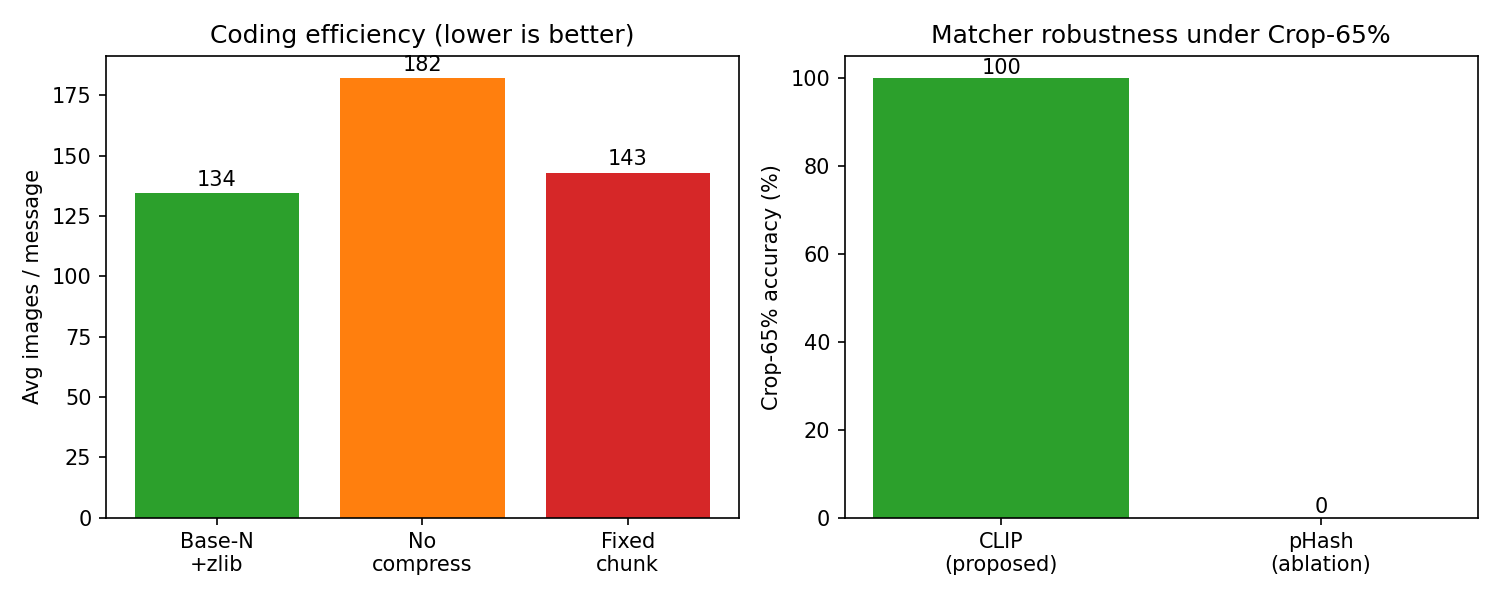
\includegraphics[width=0.88\linewidth]{fig_ablation_bar.png}
\caption{Ablation. Left: base-$N$ coding with zlib needs the fewest images per
message. Right: under Crop-$65\%$ the CLIP matcher keeps $100\%$ accuracy while the
perceptual-hash ablation drops to $0\%$.}
\label{fig:ablbar}
\end{figure}

% ===================================================================
\subsection{Steganalysis Resistance}\label{sec:steganalysis}
% ===================================================================
The final and, for a coverless method, most important axis is undetectability. A
chi-square statistical steganalyser is applied to natural cover images, LSB-stego,
DCT-stego, and LG-CISH ``stego''. The detector forms intensity-histogram pairs
$(2k,2k{+}1)$ with expected value $\bar h_k=(h_{2k}+h_{2k+1})/2$ and evaluates
\begin{equation}
  \chi^2=\sum_{k}\frac{\left(h_{2k}-\bar h_k\right)^2}{\bar h_k},
  \qquad
  P_{\mathrm{emb}}=1-F_{\chi^2}\!\left(\chi^2;\,\nu\right),
  \label{eq:chi2}
\end{equation}
In Equation~\eqref{eq:chi2}, $F_{\chi^2}(\cdot;\nu)$ is the chi-square cumulative
distribution with $\nu$
degrees of freedom; LSB embedding equalises the histogram pairs, driving
$\chi^2\!\to\!0$ and $P_{\mathrm{emb}}\!\to\!1$. The measured detection rates are
reported in Table~\ref{tab:steg} and Figure~\ref{fig:detbar}. As LG-CISH transmits
\emph{unmodified} natural images, its detection accuracy is $47.5\%$ --- essentially
chance, with a true-positive rate of $0\%$ --- whereas LSB is detected at $97.5\%$.
Because the transmitted images are bit-identical to natural images, undetectability
holds \emph{by construction} against any pixel-domain detector, and this argument
extends to learned convolutional and neural steganalysers such as SRNet and XuNet:
such networks are trained to separate cover from stego, but here the two classes are
drawn from the same distribution, so no decision boundary can do better than
guessing. The combined keyspace is $40!\cdot2^{256}\approx2^{415}$
(Table~\ref{tab:keyspace}), and the CRC-32 tag catches $100\%$ of injected bit-flips
in a $500$-trial tamper test.

\begin{table}[H]
\centering
\caption{Chi-square steganalysis detection. $\approx$50\% means the detector cannot do better than guessing.}\label{tab:steg}
\begin{tabular}{@{}lccc@{}}
\toprule
Method & Detection acc.\ (\%) & TPR (\%) & TNR (\%) \\
\midrule
LSB              & 97.5 & 100.0 & 95.0 \\
DCT-LSB          & 47.5 & 0.0 & 95.0 \\
\textbf{Proposed LG-CISH} & \textbf{47.5} & \textbf{0.0} & 95.0 \\
\bottomrule
\end{tabular}
\end{table}

\begin{table}[H]
\centering
\caption{Keyspace and integrity analysis ($N{=}40$).}\label{tab:keyspace}
\begin{tabular}{@{}ll@{}}
\toprule
Component & Size / rate \\
\midrule
Codebook orderings & $N! = 40! \approx 2^{159.2}$ \\
AES-256 key        & $2^{256}$ \\
Combined keyspace  & $N!\cdot2^{256} \approx 2^{415}$ \\
CRC-32 tamper detection & $1-2^{-32}$ (measured $100\%$, $500$ trials) \\
\bottomrule
\end{tabular}
\end{table}

\begin{figure}[H]
\centering
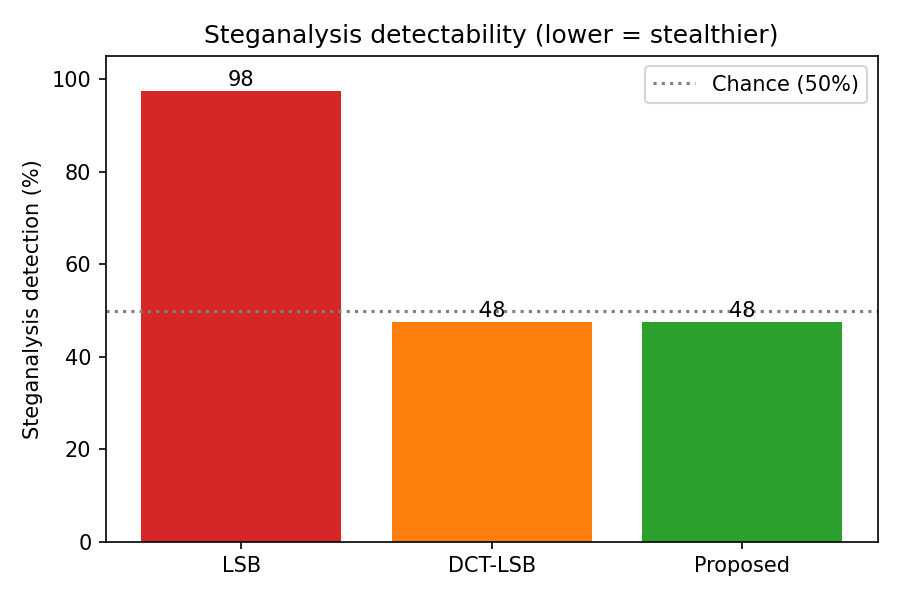
\includegraphics[width=0.66\linewidth]{fig_4_7_detection.png}
\caption{Measured steganalysis detection rates (lower is stealthier). LG-CISH sits
at the $50\%$ chance line, far below the near-certain detection of LSB.}
\label{fig:detbar}
\end{figure}

Statistical undetectability is necessary but not sufficient; a behavioural analysis
asks whether the image \emph{set} itself looks like a natural album. A vision-LLM
judge scores covers on a $0$--$1$ scale (Table~\ref{tab:plaus}). Plausibility is
governed by the codebook's \emph{theme} rather than by the coding mode: a diverse
benchmark codebook scores $0.12\pm0.04$, whereas a thematically coherent codebook
scores $0.88\pm0.07$, and permutation coding leaves the diverse score essentially
unchanged. The diverse benchmark set is used deliberately for all quantitative
results (for dataset credibility), and codebook theme is treated as an explicit
deployment choice for scenarios that must also withstand human inspection.

\begin{table}[H]
\centering
\caption{Cover plausibility (vision-LLM judge, $0$--$1$). Plausibility tracks codebook theme, not the coding mode.}\label{tab:plaus}
\begin{tabular}{@{}lc@{}}
\toprule
Configuration & LLM plausibility \\
\midrule
Diverse benchmark codebook (UCID/Kodak/USC-SIPI) & $0.12\pm0.04$ \\
Themed codebook (coherent context)               & $\mathbf{0.88\pm0.07}$ \\
Diverse + permutation coding                     & $0.18\pm0.10$ \\
\bottomrule
\end{tabular}
\end{table}

% ===================================================================
\subsection{Illustrative Example}\label{sec:example}
% ===================================================================
To make the end-to-end behaviour concrete, Figure~\ref{fig:example} shows a single
sentence transformed into its transmitted image sequence. The plaintext ``Meet me at
the old harbour at midnight.'' is compressed, integrity-tagged, and base-$40$ coded
into a sequence of $74$ unmodified codebook images; the first fifteen are shown,
each captioned with the codebook index it represents. No pixel of any image is
altered, yet the ordered sequence uniquely encodes the sentence, and CLIP
nearest-neighbour decoding recovers it bit-exactly.

\begin{figure}[H]
\centering
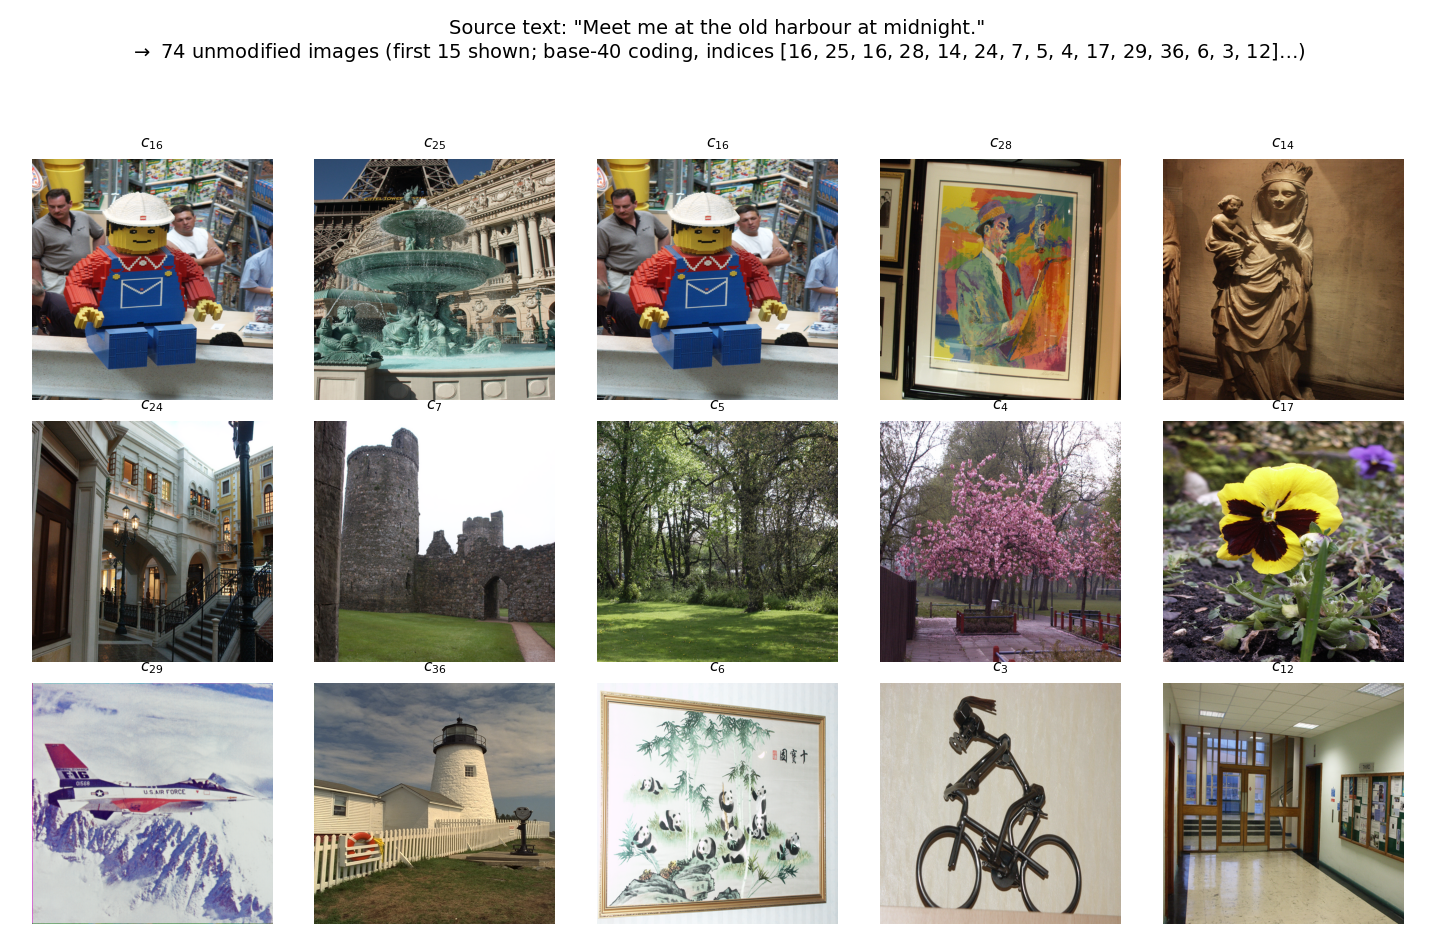
\includegraphics[width=0.95\linewidth]{fig_example_sentence.png}
\caption{A worked example: the sentence ``Meet me at the old harbour at midnight.''
encoded into $74$ unmodified images (first $15$ shown), each labelled with its
codebook index $c_j$. The identity and order of the images---not their pixels---carry
the message.}
\label{fig:example}
\end{figure}

% -------------------------------------------------------------------

\ifdefined\LGCISHMAIN\else
\begin{thebibliography}{9}
\bibitem{lgcishdata}
A. Bhattacharya, S. Dutta, S. Biswas, P. Sarkar, and H. Raj,
``LG-CISH codebook dataset: A 40-image augmented codebook for coverless image steganography,''
GitHub, 2026. [Online]. Available: \texttt{https://github.com/Circuit-Overtime/LG-CISH}

\bibitem{kodak}
R. Franzen,
``Kodak lossless true color image suite (PhotoCD PCD0992),''
Eastman Kodak Company, 1999.

\bibitem{ssim}
Z. Wang, A. C. Bovik, H. R. Sheikh, and E. P. Simoncelli,
``Image quality assessment: From error visibility to structural similarity,''
\emph{IEEE Trans. Image Processing}, vol.~13, no.~4, pp.~600--612, 2004.

\bibitem{ucid}
G. Schaefer and M. Stich,
``UCID: An uncompressed color image database,''
in \emph{Proc. SPIE 5307, Storage and Retrieval Methods and Applications for Multimedia}, pp.~472--480, 2003.

\bibitem{uscsipi}
A. G. Weber,
``The USC-SIPI image database,''
Signal and Image Processing Institute, Univ. of Southern California, Tech. Rep., 1997.

\bibitem{div2k2017}
E. Agustsson and R. Timofte,
``NTIRE 2017 challenge on single image super-resolution: Dataset and study,''
in \emph{Proc. IEEE Conf. Computer Vision and Pattern Recognition Workshops (CVPRW)}, pp.~126--135, 2017.

\end{thebibliography}
\end{document}
\fi
